%% LaTeX-Beamer template for KIT design
%% by Erik Burger, Christian Hammer
%% title picture by Klaus Krogmann
%%
%% version 2.1
%%
%% mostly compatible to KIT corporate design v2.0
%% http://intranet.kit.edu/gestaltungsrichtlinien.php
%%
%% Problems, bugs and comments to
%% burger@kit.edu

\documentclass[18pt]{beamer}

\usepackage[utf8]{inputenc}
\usepackage[babel,german=quotes]{csquotes}
\usepackage{graphicx}
\usepackage{caption}
\usepackage{subfig}
\usepackage[right]{eurosym}
\usepackage{listings}

\usepackage{booktabs}

%% SLIDE FORMAT

% use 'beamerthemekit' for standard 4:3 ratio
% for widescreen slides (16:9), use 'beamerthemekitwide'

\usepackage{templates/beamerthemekit}
% \usepackage{templates/beamerthemekitwide}


\usepackage{multirow}


% inserted by Koios to hide comments in lstlistings
\newcommand{\none}[1]{}

\lstset{language=C++, basicstyle=\footnotesize, numbers=left, numberstyle=\tiny\color{gray}, tabsize=4, xleftmargin=2em, rangeprefix=/*$\ , rangesuffix=\ $*/, includerangemarker=false, morecomment=[is]{/*$}{$*/}}


%% TITLE PICTURE

% if a custom picture is to be used on the title page, copy it into the 'logos'
% directory, in the line below, replace 'mypicture' with the 
% filename (without extension) and uncomment the following line
% (picture proportions: 63 : 20 for standard, 169 : 40 for wide
% *.eps format if you use latex+dvips+ps2pdf, 
% *.jpg/*.png/*.pdf if you use pdflatex)

\titleimage{title}

%% TITLE LOGO

% for a custom logo on the front page, copy your file into the 'logos'
% directory, insert the filename in the line below and uncomment it

\titlelogo{titlelogo}

% (*.eps format if you use latex+dvips+ps2pdf,
% *.jpg/*.png/*.pdf if you use pdflatex)

%% TikZ INTEGRATION

% use these packages for PCM symbols and UML classes
% \usepackage{templates/tikzkit}
% \usepackage{templates/tikzuml}

% the presentation starts here

\title[C++ Workshop]{C++ Workshop}
\subtitle{9. Block, 29.06.2012}
\author{Sven Brauch, Markus Jung, Oliver Schneider, Robert Schneider}

\institute{}

\begin{document}

% change the following line to "ngerman" for German style date and logos
\selectlanguage{ngerman}

\AtBeginSection[]{%
	\begin{frame}
		\tableofcontents[sectionstyle=show/hide,subsectionstyle=hide/show/hide]
	\end{frame}
	\addtocounter{framenumber}{-1}% If you don't want them to affect the slide number
}

%title page
\begin{frame}
\titlepage
\end{frame}

%table of contents
\begin{frame}{Gliederung}
\tableofcontents
\end{frame}

%%%%%%%%%%%%%%%%%%%%%%%%%
% ADD OWN SECTIONS HERE %
%%%%%%%%%%%%%%%%%%%%%%%%%
%\include{cpp} % includes cpp.tex

\section{Literale}
\begin{frame}{Literale}
    \begin{block}{Was ist ein Literal?}
    Literale sind Bestandteil der Syntax der meisten Sprachen, die dazu dienen, Daten direkt in den Quellcode zu schreiben.
    \end{block}
    \pause
    \begin{block}{Beispiele für Literale in C++}
    \begin{table}
    \center
    \begin{tabular}{ll}
        \toprule
        Typ & Beispiel \\
        \midrule
        char & 'A' \\
        const char[] (char-Array, Null-terminiert!) & "Hello World!" \\
        int & 42 \\
        double & 1.6e-19 \\
        \bottomrule
    \end{tabular}
    \caption{Literale in C++}
    \end{table}
    \end{block}
\end{frame}

\begin{frame}{Escape-Sequenzen}
    \begin{block}{Escape-Sequenzen in String-Literalen in C++}
    \begin{table}
    \center
    \begin{tabular}{ll}
        \toprule
        Sequenz & Wirkung \\
        \midrule
        \textbackslash n & Neue Zeile \\
        \textbackslash t & Tabulator \\
        \textbackslash\textbackslash & Backslash (\textbackslash) \\
        \textbackslash" & Doppeltes Anführungszeichen (") \\
        \textbackslash' & Einfaches Anführungszeichen (') \\
        \bottomrule
    \end{tabular}
    \end{table}
    \end{block}
\end{frame}

\begin{frame}{Weniger häufig genutzte Literale}
    \begin{block}{Weitere Beispiele für Literale}
        \begin{table}
        \center
        \begin{tabular}{ll}
            \toprule
            Typ & Beispiel \\
            \midrule
            Oktalzahl (int) & 042 \\
            Hexadezimalzahl (int) & 0x732 \\
            \midrule
            \pause
            unsigned int & 42u \\
            unsigned int, Oktal & 042u \\
            \midrule
            \pause
            C++11: Benutzerdefiniert & 42.7\_meter \\
            \bottomrule
        \end{tabular}
        \caption{Weitere Literale in C++}
        \end{table}
    \end{block}
\end{frame}

\section{Strings}

\begin{frame}{Probleme mit C-Strings}
    \begin{block}{Probleme mit C-Strings}
    \begin{itemize}
    \item Schwierige Handhabung, z.\,B. wegen Null-Terminierung
    \item Keine einfache Möglichkeit, mehr als die Ascii-Zeichen zu benutzen (zum Beispiel Unicode)
    \end{itemize}
    \end{block}
\end{frame}

\begin{frame}{String-Klassen}
    \begin{block}{std::string}
    \texttt{std::string} ist die String-Klasse der Standardbibliothek. Praktische Methoden:
    \begin{itemize}
    \item \texttt{size()}
    \item \texttt{append(str)}, \texttt{insert(position, str)}
    \item \texttt{operator==(str)}
    \end{itemize}
    Anders als mit \texttt{char}-Arrays kann man also zum Beispiel Strings direkt vergleichen:
    \texttt{if ( str1 == str2 ) { ... }}
    \end{block}
\end{frame}

\begin{frame}{String-Klassen}
    \begin{block}{QString}
    \texttt{QString} ist die String-Klasse der Qt-Bibliothek\footnote{\url{http://qt-project.org/}}. Im Gegensatz zu \texttt{std::string} bietet \texttt{QString} echte Unicode-Unterstützung, und viele weitere nützliche Methoden, zum Beispiel:
    \begin{itemize}
    \item \texttt{replace(QRegExp, QString)} -- suchen und Ersetzen mit regulären Ausdrücken
    \item \texttt{repeated(int)} -- wiederholt den String einige Male
    \item \texttt{trimmed()} -- entfernt Leerzeichen vorne und hinten im String
    \end{itemize}
    \end{block}
\end{frame}

\begin{frame}{String-Klassen}
	enemy slide injection :P
	
    \begin{block}{STL und Unicode}
    Die Unicode-Unterstützung der STL steckt in den Algorithmen, nicht in \texttt{std::string}:
    \begin{itemize}
    \item \texttt{std::regex\_replace(string, regex, string)} -- suchen und Ersetzen mit regulären Ausdrücken
    \item \texttt{string+=string} -- wiederholt den String einmal (einige Male == einmal 5-zeilige Funktion)
    \item \texttt{stream>>skipws>>string} -- entfernt Leerzeichen vorne und hinten im String
	\tiny
	\item \texttt{string.substr( find\_if(string.begin(), string.end(), bind( isprint, \_1, loc), reverse\_iterator(find\_if(string.rbegin(), string.rend(), bind( isprint, \_1, loc) )} -- entfernt Leerzeichen vorne und hinten im String
    \end{itemize}
    \end{block}
\end{frame}



\begin{frame}[fragile]{"Abkürzungen" in C++}
	
	\begin{lstlisting}[]
namespace Gebaeck
{
	namespace Kuchen
	{
		struct A { int a; }
		struct B { A b; }
	}
}
Gebaeck::Kuchen::A blub;
blub.a = 99;

using namespace Gebaeck::Kuchen;

B bla;
bla.b.a = 42;
	\end{lstlisting}
\end{frame}

\begin{frame}[fragile]{"Abkürzungen" in C++}
	Problem: 5 namespaces mit struct A... welchen nutzen?

	\begin{lstlisting}[]
namespace Gebaeck
{
	namespace Kuchen
	{
		struct A { int a; }
		struct B { A b; }
	}
}
using C = Gebaeck::Kuchen::B;

C meinC;
C.b.a = 273;
	\end{lstlisting}
\end{frame}



\section{Etwas mehr zu templates}

\begin{frame}[t]{template argument deduction}
	Bei einem \enquote{Aufruf eines function templates} kann der Compiler (manche) template-Argumente anhand der Typen der function-call-Argumente bestimmen:
	
	\onslide*<+> { \lstinputlisting[linerange=begin-deduction]{cpp-code/type-deduction.cpp} }
	\onslide<+-> { \lstinputlisting[linerange=begin-]{cpp-code/type-deduction.cpp} }
\end{frame}

\begin{frame}[t]{non-type template parameters}
	Bisher: Typen als Parameter der Vorlage\\
	\onslide<2> { Jetzt neu: z.B. \texttt{int} als Parameter der Vorlage }
	
	\onslide*<1> { \lstinputlisting[linerange=int-instantiation]{cpp-code/non-type-template-parameters.cpp} }
	\onslide<2> { \lstinputlisting[linerange=int-]{cpp-code/non-type-template-parameters.cpp} }
\end{frame}

\begin{frame}{non-type template parameters: constraints}
	Der Wert muss eine constant-expression sein, also dem Compiler bekannt!	\\
	Denn sonst kann dieser das Template nicht Instantiieren.
	
	\vspace{2em}
	
	Erlaubte Typen:
	\begin{itemize}
		\item integral
		\item enumeration
		\item exotisch: Referenz oder Poiniter zu »Ding« \emph{mit external linkage}
		\item kein String!
	\end{itemize}
\end{frame}

\begin{frame}[fragile]{Iteratoren in C++}
	\begin{itemize}
		\item Einheitlicher Zugriff auf alle STL-Container
		\item Dadurch Algorithmen leicht auf unterschiedliche Container anzuwenden
		\item Notwendig für Container ohne Random Access (list)
		\item Praktisch für Assoziative container (set, map)
	\end{itemize}
\end{frame}

\begin{frame}[fragile]{Iteratoren in C++}
	
	\begin{lstlisting}[]
#include <list>
using intList = std::list<int>;
using intIt = intList::iterator;
intList meineListe;
meineListe.push_back(42);
meineListe.push_back(1024);
meineListe.push_front(1);

for(intIt it = meineListe.begin(); it != meineListe.end(); it++)
{
	std::cout << *it << std::endl;
}
for(int i : meineListe)
{
	std::cout << i << std::endl;
}
	\end{lstlisting}
\end{frame}

\section{STL-Datenstrukturen}

\subsection{container adaptors}

\begin{frame}{Überblick - container adaptors}
 	\begin{block}{Adapter (Entwurfsmuster)}
	 	\pause
	 	Ausgangssituation: Eine Klasse bietet den erforderlichen Funktionsumfang, aber nicht (genau) die gewünschte Schnittstelle.
	 	
	 	\pause
	 	
	 	Ein Adapter:
	 	\begin{itemize}
	 		\item Übersetzt eine inkompatible Schnittstelle
	 		\item Wandelt ggf. die verwendeten Datenformate um
	 		\item Ist nach außen hin nicht als ein solcher erkennbar
	 	\end{itemize}
 	\end{block}
 	
 	\pause
 	
	\begin{itemize}
		\item \texttt{stack}
		\item \texttt{queue}
		\item \texttt{priority\_queue}
	\end{itemize}
	
	\pause
	
	\texttt{stack} und \texttt{queue} sind schon fast mehr Interface als eine vollwertige Klasse. Reicht deren Funktionsumfang aus, darf daher gerne deren Schnittstelle genutzt werden, was mehr Wahlfreiheit bei der Auswahl der zugrundeliegenden Datenstruktur erlaubt.
\end{frame}

\begin{frame}{\texttt{stack}}
	\begin{columns}
		\column{.3\linewidth}
			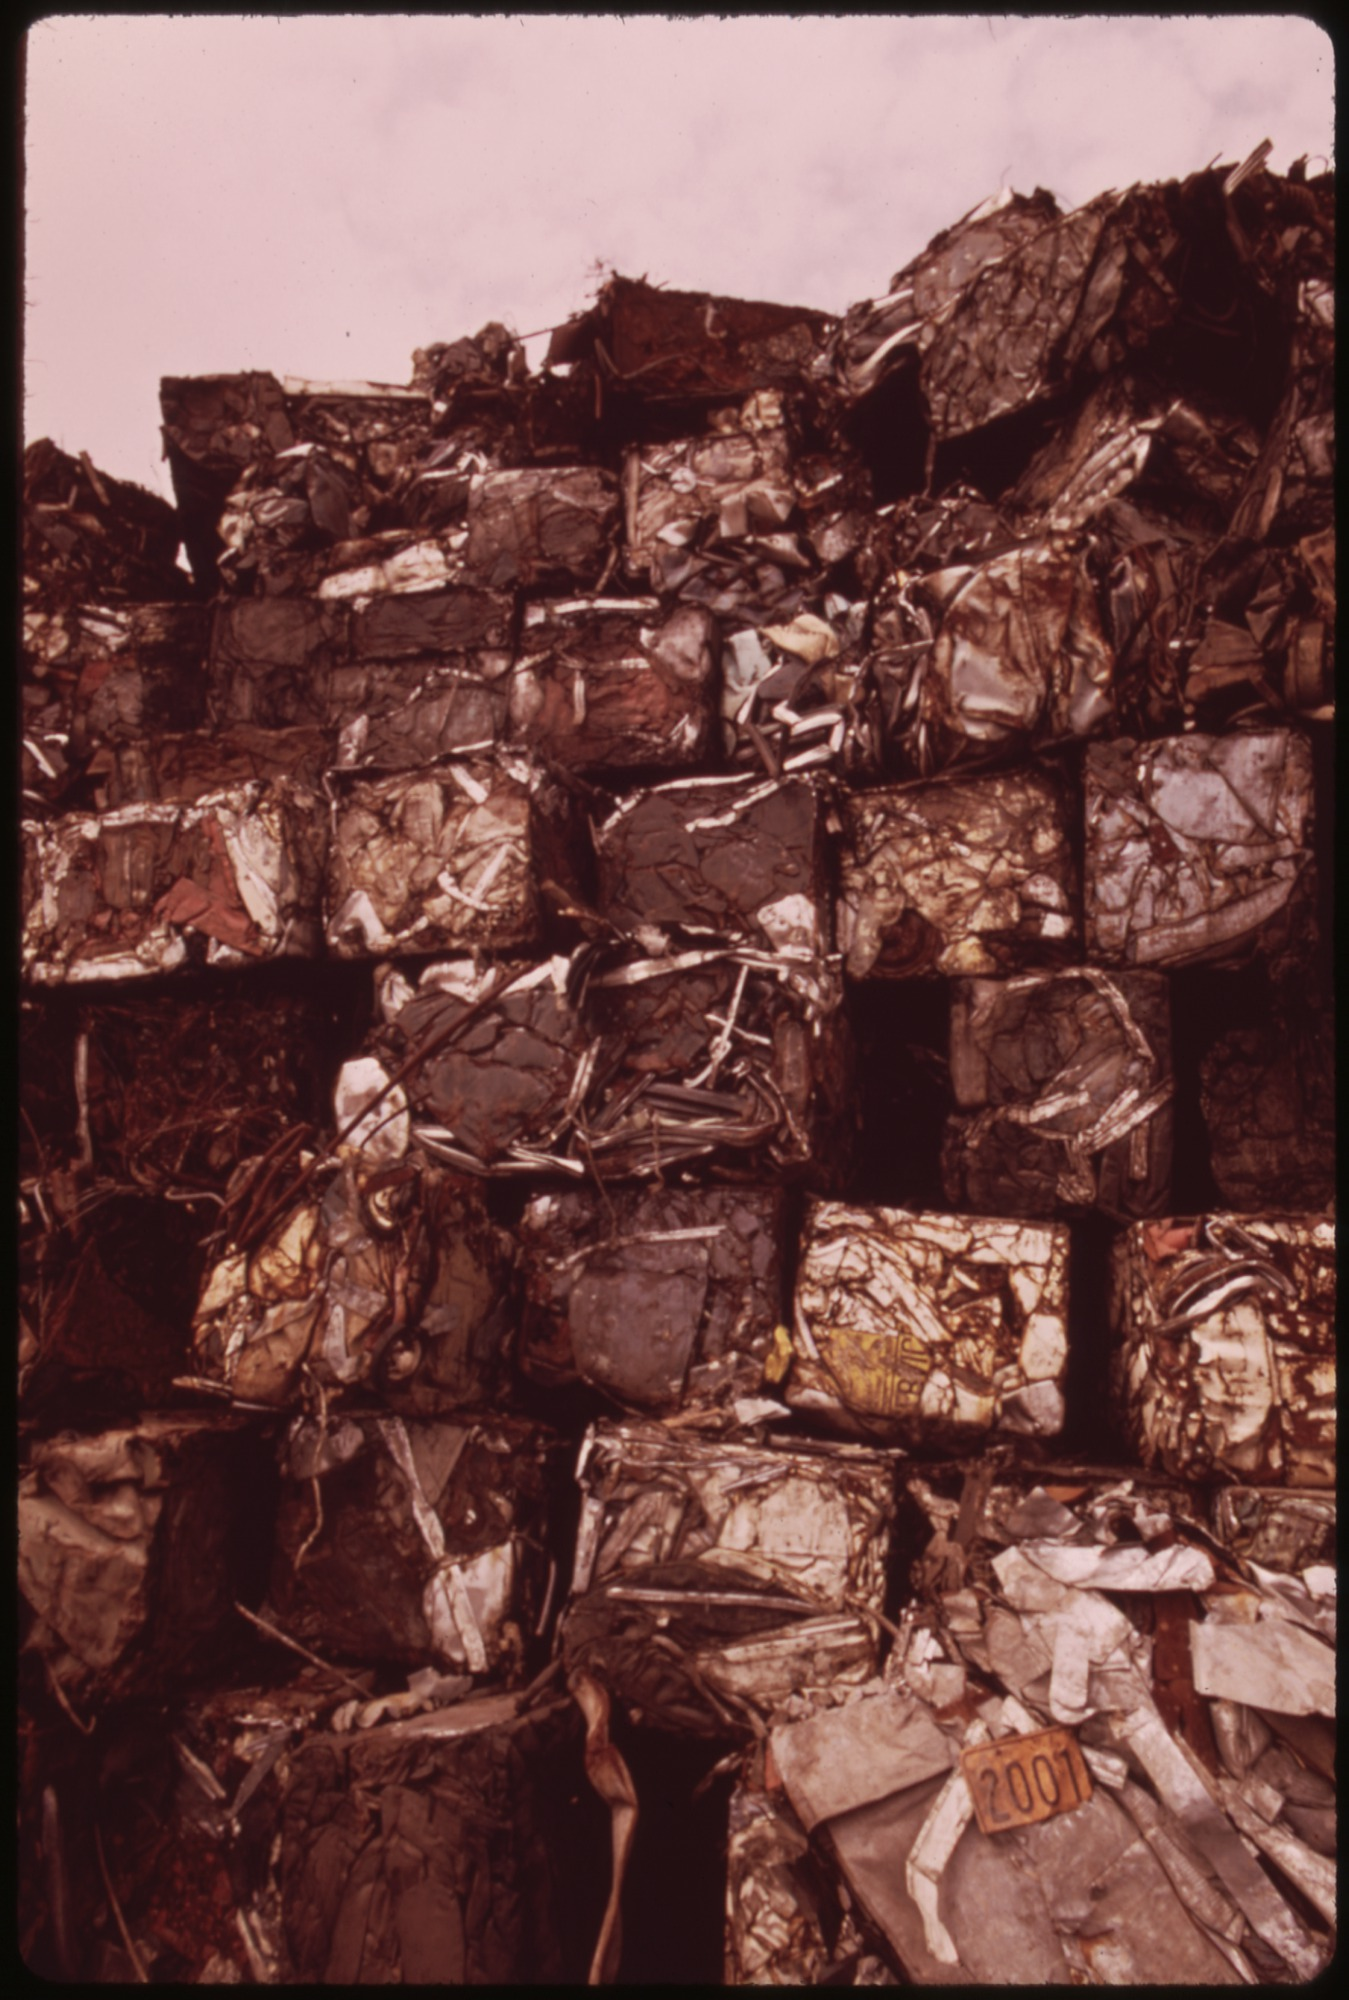
\includegraphics[width=\linewidth]{images/stack.jpg}
			
		\column{.7\linewidth}
			\begin{itemize}
				\item Kann mit \texttt{deque}, \texttt{list} und \texttt{vector} arbeiten
				\item Wichtig: \texttt{top()}, \texttt{push()} und \texttt{pop()}
				\item Laufzeit: $\mathcal{O}(1)$ für alle Einzel-Operationen
			\end{itemize}
			
			\vspace{1em}
			
			\begin{itemize}
				\item Einsatz: Bei Bedarf
			\end{itemize}
	\end{columns}
\end{frame}

\begin{frame}{\texttt{queue}}
	\begin{center}
		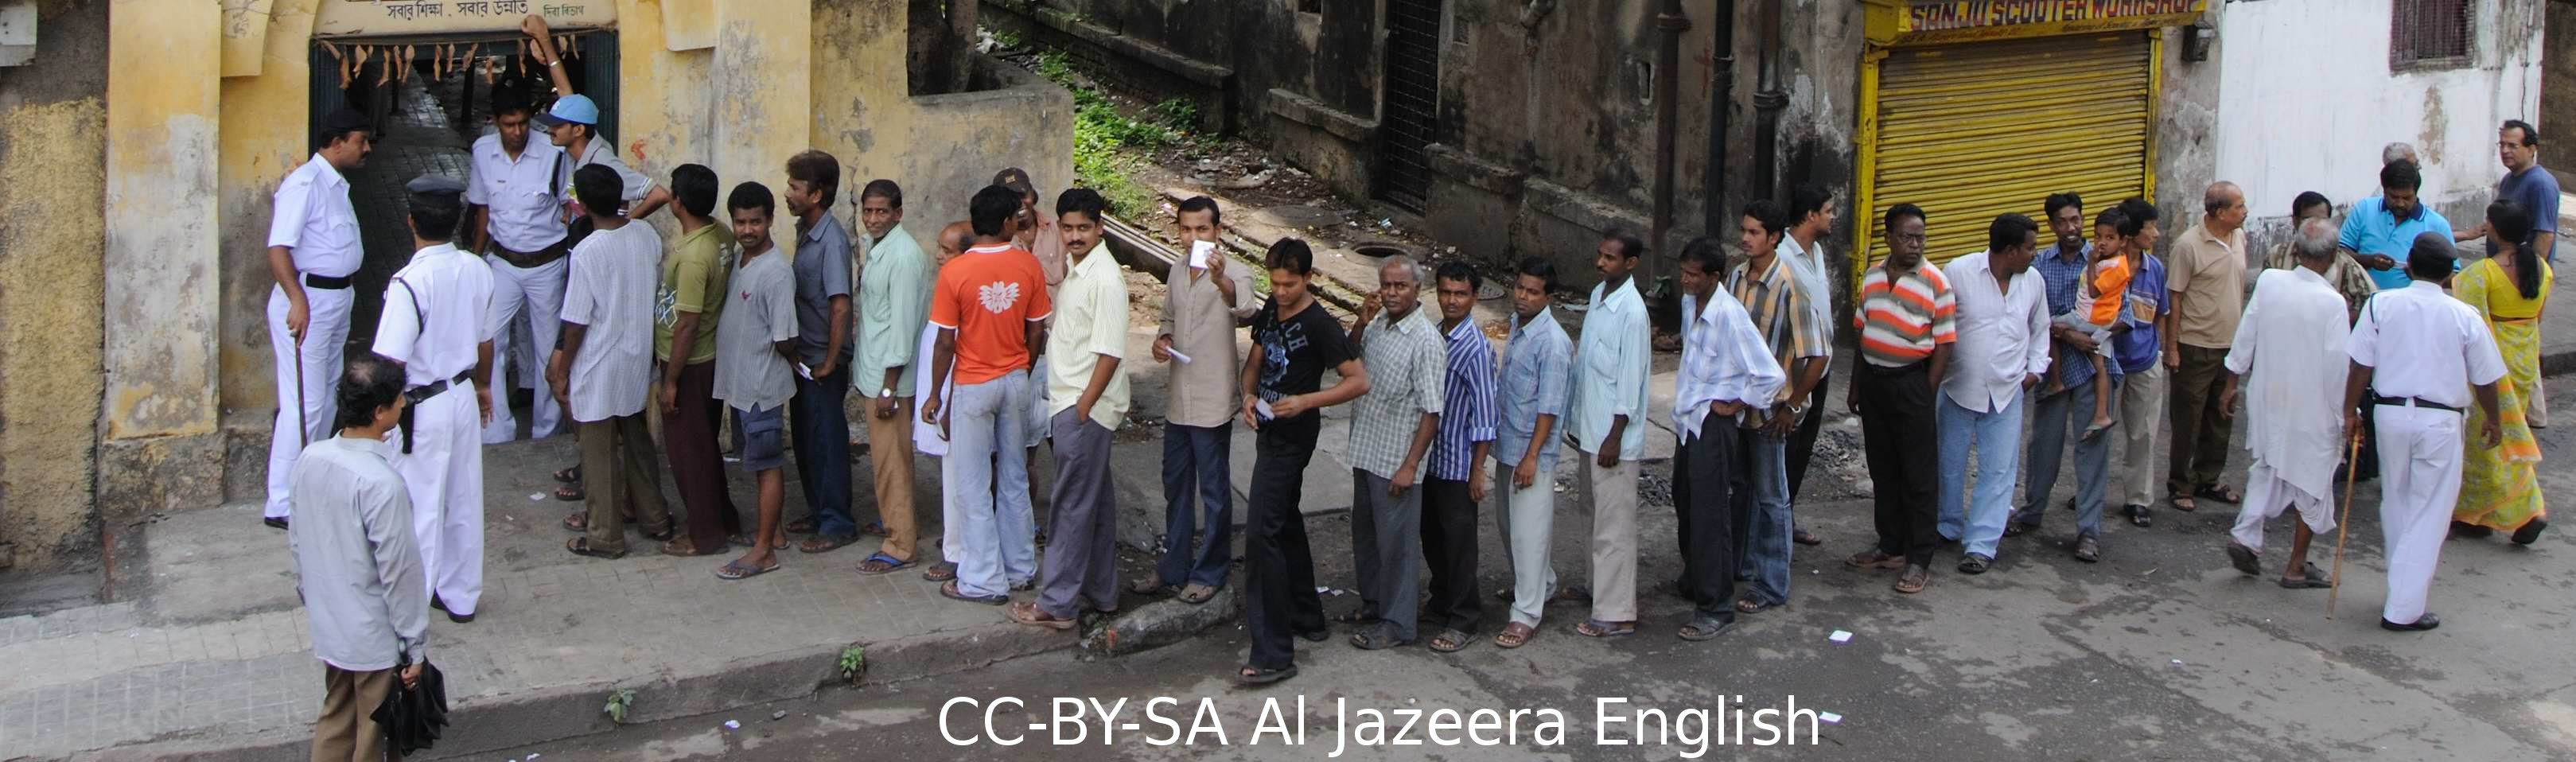
\includegraphics[width=0.7\linewidth]{images/queue.jpg}
	\end{center}
	
	\begin{itemize}
		\item Kann mit \texttt{deque} und \texttt{list} arbeiten, aber nicht mit \texttt{vector}
		\begin{itemize}
			\item \alert{Warum?}
			\pause
			\item Weil entfernen am Anfang eines \texttt{vector} \enquote{teuer} ($\mathcal{O}(n)$) ist
		\end{itemize}
		\item Wichtig: \texttt{front()}, \texttt{back()}, \texttt{push()} und \texttt{pop()}
		\item Laufzeit: $\mathcal{O}(1)$ für alle Einzel-Operationen
	\end{itemize}
	
	\begin{itemize}
		\item Einsatz: Bei Bedarf
	\end{itemize}
\end{frame}

\begin{frame}{Prioritätslisten (Priority Queues)}
	\begin{block}{Was?}
		\begin{itemize}
			\item Menge von Elementen mit einem Schlüssel
			\item Geordnet nach Schlüssel (Ordnungsrelation: $\le$)
			\item Wichtigste Operationen: 
			\begin{itemize}
				\item \texttt{insert(key, value)} 
				\item \texttt{deleteMin()} \tiny{(Alternativ: \texttt{deleteMax()}) $\rightarrow$ MinHeap/MaxHeap}
			\end{itemize}
			\item Für viele Algorithmen nützlich
		\end{itemize}
	\end{block}
	\pause
	\begin{block}{Wie?}
		\begin{columns}
			\column{0.7\linewidth}
				\vspace{-0.5em}
				\begin{itemize}
					\item Binäre Heaps
					\begin{itemize}
						\item Baumstruktur
						\item Jeder Knoten hat 0..2 Kindknoten
						\item Keine Löcher, Fehlstellen nur rechtsseitig
						\item Tiefe: $\lfloor log_2(n) \rfloor$
					\end{itemize}
					\item Heap-Eigenschaft: Elternknoten $\le$ Kindknoten
				\end{itemize}
			\column{0.3\linewidth}
				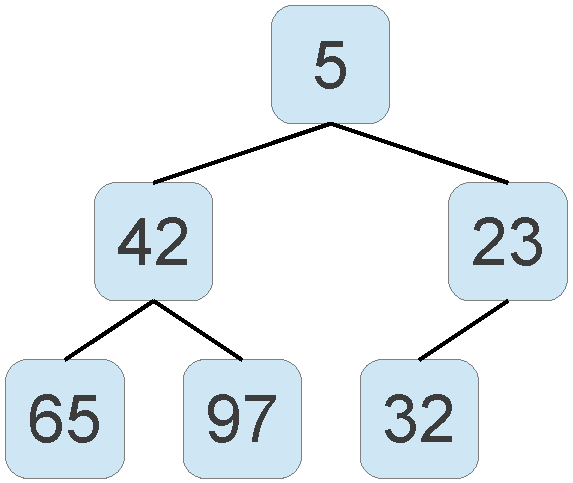
\includegraphics[width=0.95\linewidth]{images/heap.pdf}
		\end{columns}
	\end{block}
\end{frame}

\begin{frame}{Binäre Heaps: \texttt{insert()}}
	\begin{center}
		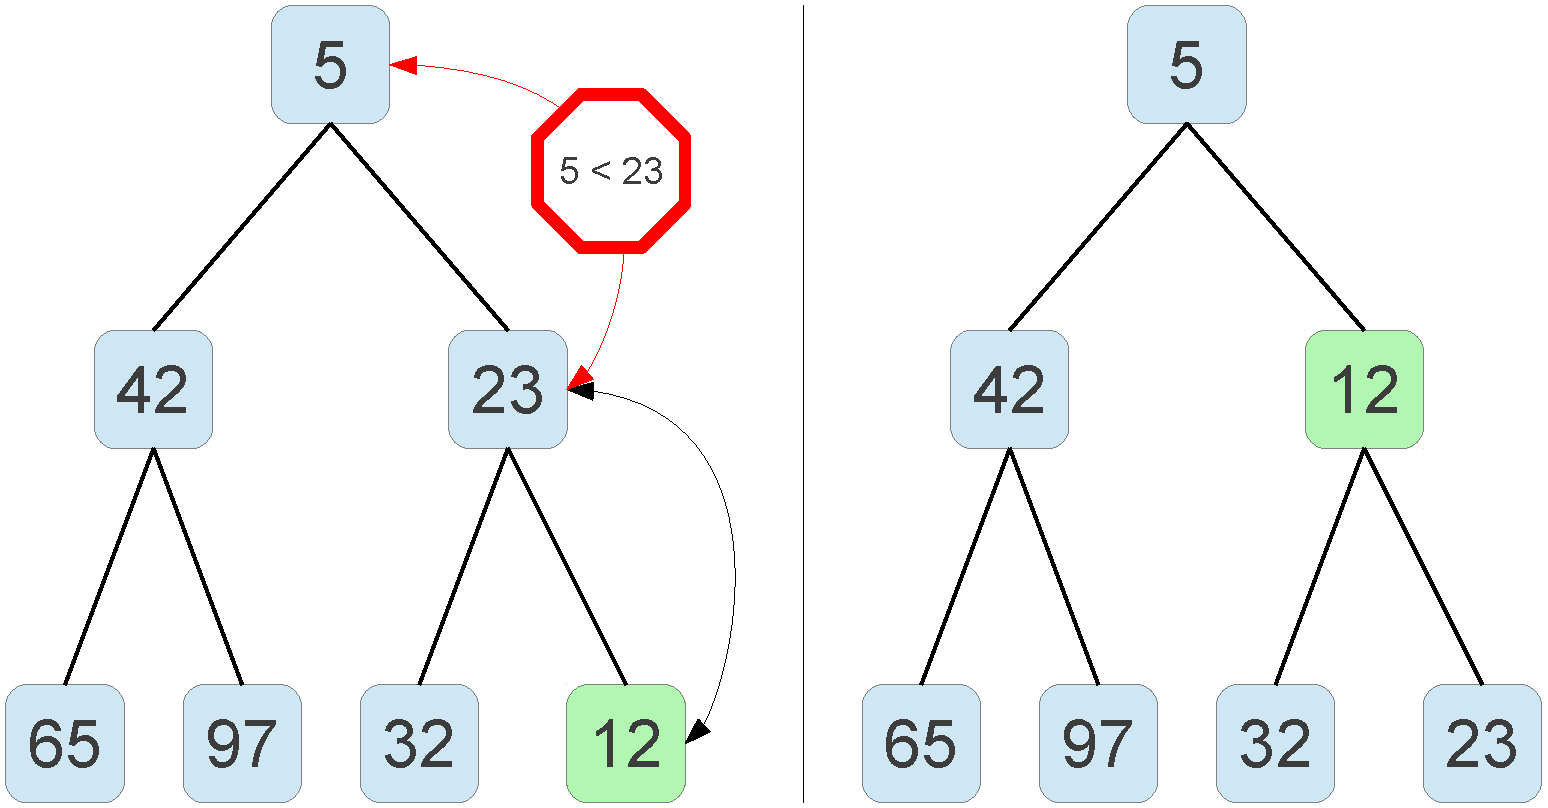
\includegraphics[width=0.90\linewidth]{images/heap_insert.pdf}
	\end{center}
\end{frame}

\begin{frame}{Binäre Heaps: \texttt{deleteMin()}}
	\begin{center}
		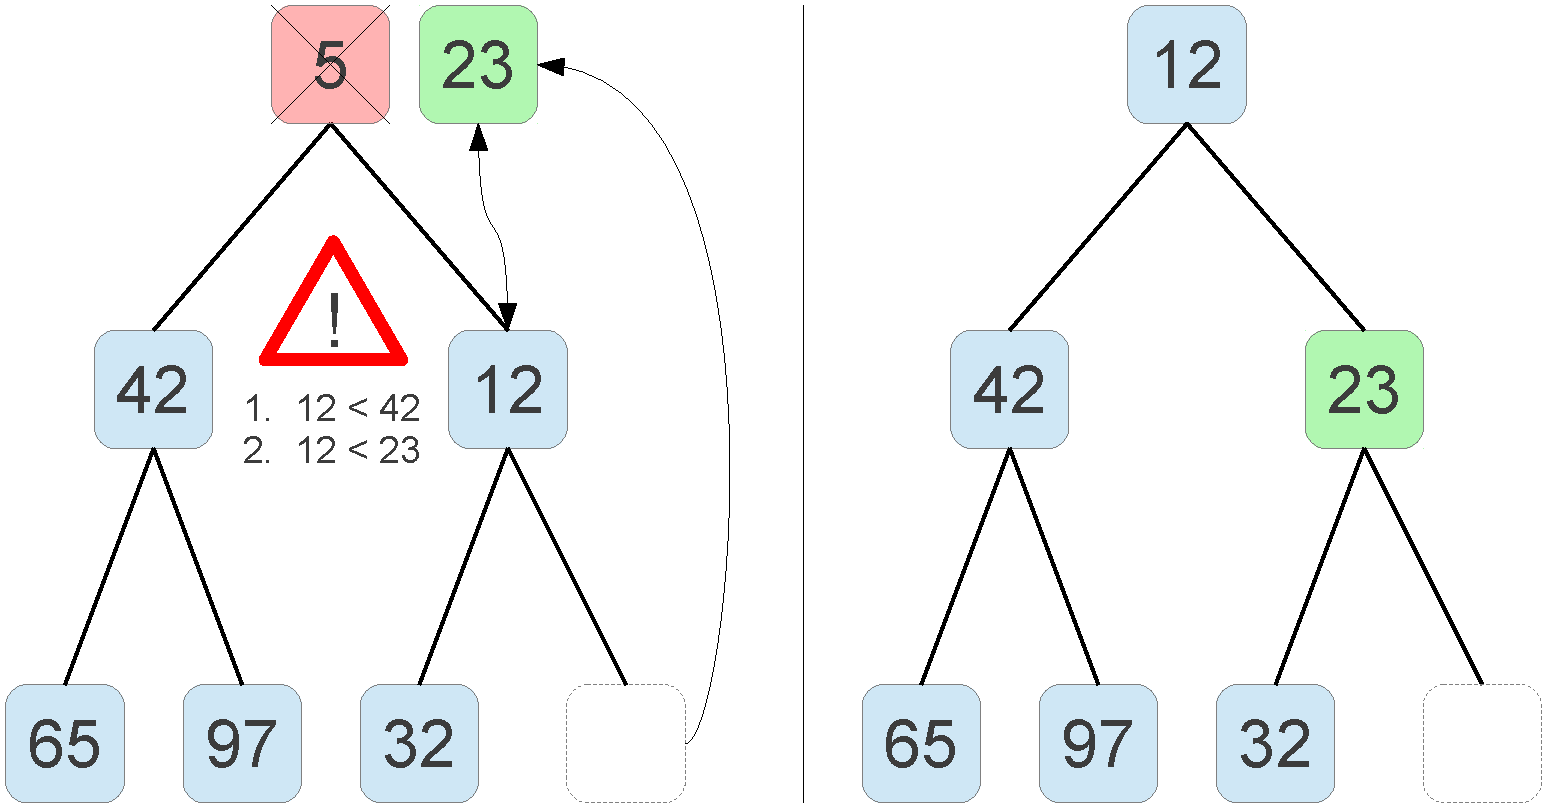
\includegraphics[width=0.90\linewidth]{images/heap_delete.pdf}
	\end{center}
\end{frame}

\begin{frame}{Binäre Heaps: Einbettung}
	\begin{center}
		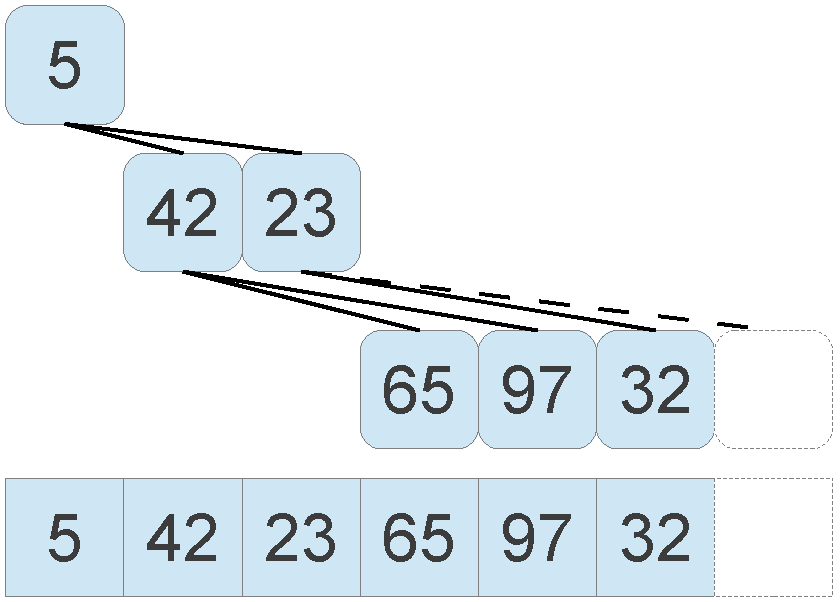
\includegraphics[width=0.85\linewidth]{images/heap_embed.pdf}
	\end{center}
\end{frame}

\begin{frame}{\texttt{priority\_queue}}
	\begin{itemize}
		\item Kann mit \texttt{deque} und \texttt{vector} arbeiten, aber nicht mit \texttt{list}
		\begin{itemize}
			\item \alert{Warum?}
			\pause
			\item Einbettung: Größere Sprünge beim Traversieren $\rightarrow$ \enquote{teuer} ($\mathcal{O}(n)$)
		\end{itemize}
		\item Wichtig: \texttt{top()}, \texttt{push()} und \texttt{pop()}
		\pause
		\item Laufzeit: $\mathcal{O}(log(n))$ für Modifikationen
		\item Heap-Eigenschaft hier: child @ parent (@ : Vergleichsoperator)
	\end{itemize}
	
	\pause
	
	\lstinputlisting[basicstyle=\scriptsize]{cpp-code/pq-usage.cpp}
\end{frame}

\subsection{associative containers}

\begin{frame}{Überblick}
	\begin{block}{Assoziative Container?!}
	 	\begin{itemize}
	 		\item Erweiterung der \texttt{priority\_queue}: Zugriff über Schlüssel
	 		\item Universell einsetzbar
	 	\end{itemize}
 	\end{block}
 	
 	\pause
 	
	\begin{itemize}
		\item \texttt{(multi)map}
		\item \texttt{(multi)set}
	\end{itemize}
\end{frame}

\begin{frame}{Sortierte Folgen}
	\begin{itemize}
		\item Zuordnung Schlüssel $\rightarrow$ Element
		\item Speicherung: Geordnet nach Schlüssel
	\end{itemize}
	\begin{center}
		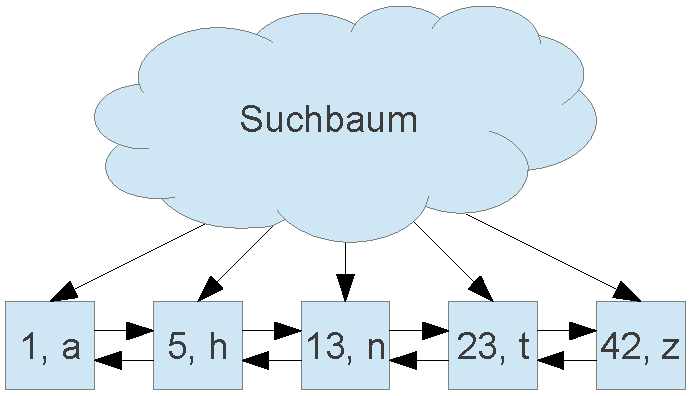
\includegraphics[width=0.7\linewidth]{images/sorted_sequence.pdf}
	\end{center}
\end{frame}

\begin{frame}{\texttt{(multi)map}}
	\begin{itemize}
		\item \texttt{multimap}: Erlaubt mehr als ein Element je Schlüsselwert
		\item Schlüssel + Element: \texttt{pair<key\_t, value\_t>}
		\pause
		\item Wichtige Operationen:
		\begin{itemize}
			\item \texttt{find(key\_t)}
			\item \texttt{operator[key\_t]}
			\item \texttt{insert(pair<\dots>)}, \texttt{erase(key\_t)}
			\item \texttt{lower\_bound(key\_t)}, \texttt{upper\_bound(key\_t)}
		\end{itemize}
		\pause
		\item Zeitkomplexität: Meist $\mathcal{O}(log(n))$
	\end{itemize}
	
	\pause
	\lstinputlisting[basicstyle=\scriptsize]{cpp-code/map-usage.cpp}
	\pause
	
	\footnotesize
	Mehr/bessere Beispiele: \url{http://www.cplusplus.com/reference/stl/map/}
\end{frame}

\begin{frame}{\texttt{(multi)set}}
	\begin{itemize}
		\item \texttt{set<type>} == \texttt{map<type, type>}
		\item[] $\rightarrow$ Element ist gleichzeitig Schlüssel
		\pause
		\item Wichtige Operationen:
		\begin{itemize}
			\item \texttt{find()}
			\item \texttt{insert()}, \texttt{erase()}
			\item \texttt{lower\_bound()}, \texttt{upper\_bound()}
		\end{itemize}
		\pause
		\item Zeitkomplexität: Meist $\mathcal{O}(log(n))$
	\end{itemize}
\end{frame}

\subsection{bitset}

\begin{frame}{\texttt{bitset}}
	\begin{itemize}
		\item Der Name ist irreführend! Besser wäre \texttt{bitvector}
		\item Kann: Bitfolgen kompakt speichern
		\item Achtung: Die Größe ist fix (Template-Parameter)
		\begin{itemize}
			\item Im Gegensatz zu \texttt{vector<bool>}
		\end{itemize}
		\pause
		\item Wichtige Operationen:
		\begin{itemize}
			\item \texttt{set()}, \texttt{reset()} und \texttt{flip()}
			\item \texttt{test()}, \texttt{any()} und \texttt{none()}
		\end{itemize}
		\item Zeitkomplexität: $\mathcal{O}(1)$
	\end{itemize}
\end{frame}



\section{Praxis}
\begin{frame}[fragile]{Praxis!}
	\begin{itemize}
		\item Aufgabe 1: Titel
		\item Aufgabe 2: Noch ein Titel
	\end{itemize}
	\ \\
	\ \\
	\large{\url{https://github.com/kit-cpp-workshop/workshop-ss12-09}} \\
	\ \\
	Aufgabenbeschreibungen und Hinweise: Siehe \verb|README.md|

\end{frame}


\end{document}
